\documentclass[19pt,landscaoe]{article}
\usepackage[landscape]{geometry}
\geometry{a5paper,scale=0.8}
%\geometry{left=1.5cm,right=1.5cm,top=1.5cm,bottom=0.5cm}
\usepackage{color}
\usepackage{ulem} % for strikethrough
\usepackage{amsfonts}
\usepackage{bm}
\usepackage{graphicx} 
\usepackage{amsfonts,amsmath,latexsym,amssymb,mathrsfs,amsthm,mathtools}
% \usepackage[british]{babel}
%\usepackage[T1]{fontenc}
%\usepackage{mathptmx}
% \usepackage{times}
\usepackage{datetime2}
\usepackage{filemod}
% \usepackage{fontspec}    %change font 
% \setmainfont{Times New Roman}%fontspec下这个命令设置全局默认字体
\newtheorem{thm}{Theorem}%[section]
\newtheorem{prop}[thm]{Proposition}
\newtheorem{defi}[thm]{Definition}
\newtheorem{lma}[thm]{Lemma}
\newtheorem{cor}[thm]{Corollary}
\newtheorem{exam}[thm]{Example}
\newtheorem{countexam}[thm]{Counterexample}
\newtheorem{rem}[thm]{Remark}
\newtheorem{con}[thm]{Conjecture}
%\bracketfactory{floor}{\lfloor}{\rfloor}
\usepackage{enumerate}
\usepackage{color}
%\usetheme{Copenhagen}
\usepackage[english]{babel}
\usepackage[utf8x]{inputenc}
\newcommand{\law}{\mathscr{L}}
\newcommand{\HH}{\mathscr{H}}
\newcommand{\D}{\mathbb{D}}
\newcommand{\IP}{\mathbb{P}} 
\newcommand{\bone}{{\bf 1}}
\DeclareMathOperator{\E}{\mathbb{E}}
\DeclareMathOperator*{\esssup}{ess\,sup}
\newcommand{\IE}{\E}
\newcommand{\mean}{\E}
\newcommand{\R}{\mathbb{R}}
\newcommand{\N}{\mathbb{N}}
\newcommand{\non}{\nonumber}
\newcommand{\Z}{\mathbb{Z}}
\newcommand{\C}{\mathbb{C}}
%\newcommand{\C}{{\mathds{C}}}
\newcommand{\ci}{{\cal I}}
\newcommand{\cf}{{\cal F}}
\newcommand{\LL}{\textbf{L}}
\DeclareMathOperator{\Var}{\mathrm{Var}}
\DeclareMathOperator{\var}{\mathrm{Var}}
\DeclareMathOperator{\cov}{\mathrm{Cov}}
\DeclareMathOperator{\bigo}{\mathrm{O}}
\newcommand{\K}{\textbf{Ker}}
\newcommand{\Id}{\textbf{Id}}
\newcommand{\Pn}{{\rm Pn}}
\newcommand{\dtv}{{d_{\rm TV}}}
\newcommand{\dk}{{d_{\rm K}}}
\newcommand{\dw}{{d_{\rm W}}}
\def\tg{{\tilde g}}
\def\a{{\alpha}}
\def\cn{{\mathcal{N}}}
\def\equald{\stackrel{\mbox{\scriptsize{{\rm d}}}}{=}}
\def\ER{Erd\H{o}s-R\'enyi}
\usepackage{color} 
\definecolor{lightblue}{rgb}{0,0.2,0.5}
\usepackage[colorlinks=true, urlcolor=lightblue,linkcolor=lightblue, citecolor=lightblue]{hyperref}

%%%%%%%%%%%%%%%%%%%%%%%%%%%%%%%%%%

%%% Define bracket commands
\def\given{\mskip 0.5mu plus 0.25mu\vert\mskip 0.5mu plus 0.15mu}
\newcounter{@bracketlevel}
\def\@bracketfactory#1#2#3#4#5#6{
\expandafter\def\csname#1\endcsname##1{%
\addtocounter{@bracketlevel}{1}%
\global\expandafter\let\csname @middummy\alph{@bracketlevel}\endcsname\given%
\global\def\given{\mskip#5\csname#4\endcsname\vert\mskip#6}\csname#4l\endcsname#2##1\csname#4r\endcsname#3%
\global\expandafter\let\expandafter\given\csname @middummy\alph{@bracketlevel}\endcsname
\addtocounter{@bracketlevel}{-1}}%
}
\def\bracketfactory#1#2#3{%
\@bracketfactory{#1}{#2}{#3}{relax}{0.5mu plus 0.25mu}{0.5mu plus 0.15mu}
\@bracketfactory{b#1}{#2}{#3}{big}{1mu plus 0.25mu minus 0.25mu}{0.6mu plus 0.15mu minus 0.15mu}
\@bracketfactory{bb#1}{#2}{#3}{Big}{2.4mu plus 0.8mu minus 0.8mu}{1.8mu plus 0.6mu minus 0.6mu}
\@bracketfactory{bbb#1}{#2}{#3}{bigg}{3.2mu plus 1mu minus 1mu}{2.4mu plus 0.75mu minus 0.75mu}
\@bracketfactory{bbbb#1}{#2}{#3}{Bigg}{4mu plus 1mu minus 1mu}{3mu plus 0.75mu minus 0.75mu}
}


% \title{Nonparametric Regression}
% \author{Qingwei Liu}
% \institute{National University of Singapore}
% \date{\today}

\begin{document}
% \maketitle
%

\begin{titlepage}
\begin{center}
    \vfill
\textbf{\huge ST5207 Nonparametric Regression\\
Semester 1, AY2024/25}\\[4cm]
\begin{minipage}{0.4\textwidth}
\begin{center} \large
Lecturer:~Qingwei Liu\\
% Email:liu\_qw@nus.edu.sg\\
\vskip 6pt
Department of Statistics and Data Science\\
\vskip 6pt
National University of Singapore
\end{center}
\end{minipage}%\\[1cm]
\vfill
% \includegraphics[width=0.1\textwidth]{./logo}\\[0.5cm]
\vfill
\end{center}

\end{titlepage}
%
\newpage
{\LARGE\centerline{\textbf {Administration}\footnote{Last modified in \filemodprintdate{Lecture1}.}}}
\vskip25pt
\begin{minipage}{.9\textwidth}
    \Large
\begin{itemize}
\item Course website: Accessible through \href{https://www.nus.edu.sg/canvas/login/}{Canvas} for lecture slides, assignments, solutions, etc. 
\item Prerequisites: Probability and Mathematical Statistics 
\item Consultation: via email \& appointment via email
\item a 2-hour lecture + 1-hour tutorial per week
\item Homework
\item Assessment: Final exam ($80\%$) + Assignments ($20\%$)
\item Main reference includes \cite{hardle04}, \cite{takezawa05}, \cite{Hall13}, and \cite{kloke14}.

\end{itemize}
\end{minipage}
\newpage
{\LARGE\centerline{\textbf{Lecture~1:~Introduction}}}
\vskip25pt
\begin{minipage}{.9\textwidth}
    \Large
\begin{itemize}
\item The course is about various {\it smoothing} methods for estimating the probability density functions (p.d.f.) and the conditional mean functions in regression settings.
\item {\it Smoothing} is a central idea in statistics and takes a role of extract structural elements of variable complexity from patterns of random variation. 
\item Smoothing is a ``modern'' nonparametric method of statistical inference, as it grows up after the wide-spread of modern computer power. 
\item A twin brother of the bootstrap, another computer intensive statistical
method.

\end{itemize}
\end{minipage}
\newpage
{\Large\centerline{\textbf{Parametric v.s. Nonparametric}}}
\vskip25pt
\begin{minipage}{.9\textwidth}
    \Large
Two distinct approaches of modelling and inference. 
\vskip 5pt
Let $X_1,\dots,X_n$ be a sequence of independent and identical distributed (i.i.d.) random variables with a common cumulative distribution function (c.d.f.) $F$. Alternatively, we write $X_1,\dots,X_n\overset{\mathrm{i.i.d.}}{\sim}F$. \\Assume the distribution function $F$ has a density function $$f(x)=\frac{\mathrm{d}F(x)}{\mathrm{d}x}.$$  
The parametric approach for density estimation assmues known function forms of $F$ or $f$ which involves some unknown {\bf parameters}.\\ We may write
$$F(x)=F_\theta(x)=F(x|\theta).$$
One has to make prior assumptions about its functional form.
\end{minipage}
\newpage
{\LARGE\centerline{\textbf{Pros and Cons of Parametric method}}}
\vskip25pt
\begin{minipage}{.9\textwidth}
    \Large
\begin{itemize}
\item The most popular parametric method of inference (estimation, test hypotheses and confidence intervals) is based on Fisher's maximum likelihood (ML).
\item The maximum likelihood estimation usually achieves the optimal efficiency of estimation as described by its variance property.
\item If the specified parametric model is wrong or far away from the true model, estimating the parametric model (MLE etc) may lead to very inaccurate results. 

\end{itemize}
\end{minipage}
\newpage
{\LARGE{\textbf{Parametric Modeling}}}
\vskip25pt
{\Large\bf{Examples}}
   
\begin{figure}[h]
% \begin{minipage}[t]{.4\linewidth}

    %the four numbers after "trim=" are for left bottom right top
      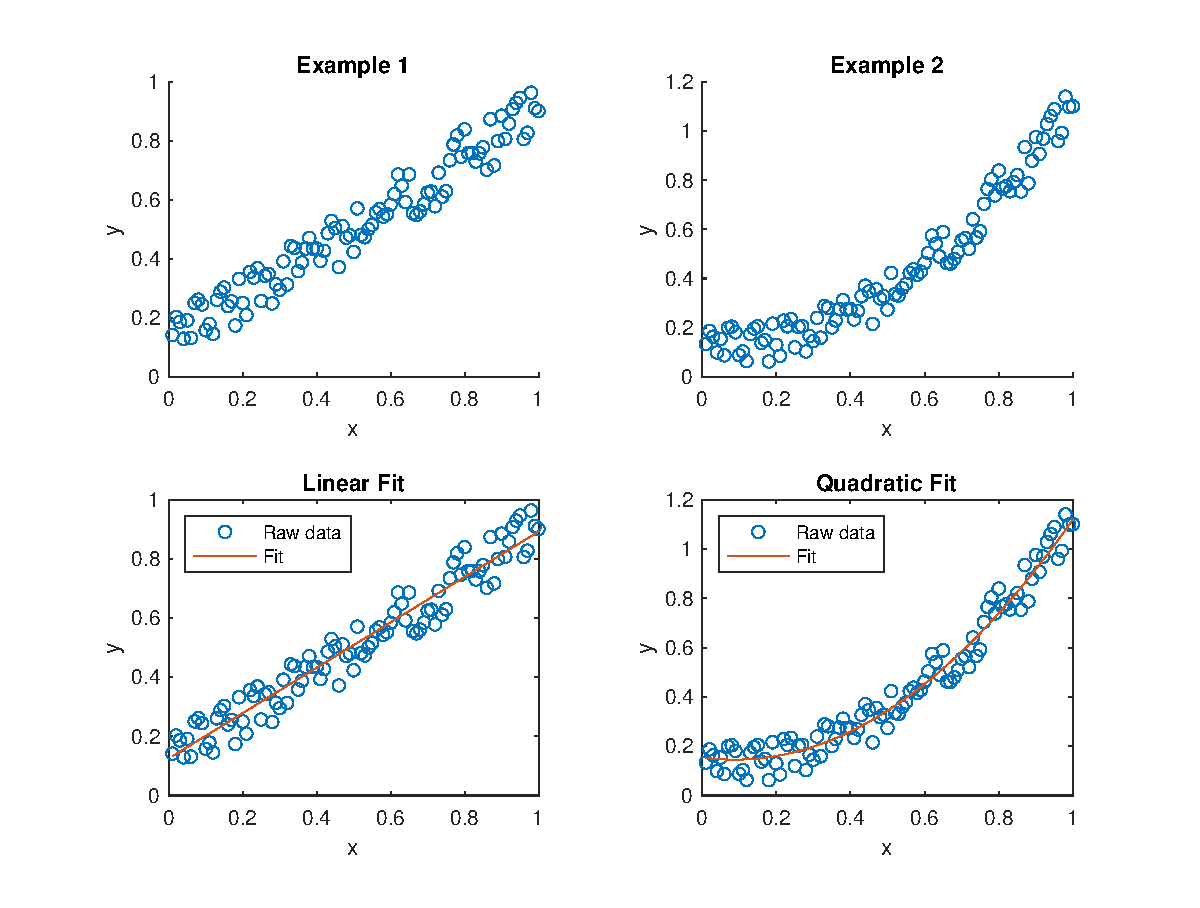
\includegraphics[width=0.8\textwidth,height=0.5\textwidth]{figure1.eps}
    %  \caption{$N(\lambda_n,\sigma_n^2)$ without correction} %
    \label{figure1} 

% \end{minipage}
\end{figure}

\newpage
{\LARGE{\textbf{Parametric Modelling}}}
\vskip25pt
\begin{minipage}{.9\textwidth}
    \Large{The motocycle date from \cite{Silverman85a}. More details about the experiment can be found in \cite{schmidt81}.}
    % \Large
\begin{itemize}
\item Collected to study the crashed effects after the motorcycles hit by a stimulated impact. 
\item Dependent variables: time after a stimulated impact with motorcycles
\item Response variables: head acceleration of a PTMO (post mortem human test object), capturing the crash effects

\end{itemize}
\end{minipage}

\newpage
{\LARGE{\textbf{Parametric Modeling}}}
\vskip25pt
{\Large\bf{Scatter plot of raw data}}

\begin{figure}[h]
% \begin{minipage}[t]{1\linewidth}
\centering
    %the four numbers after "trim=" are for left bottom right top
      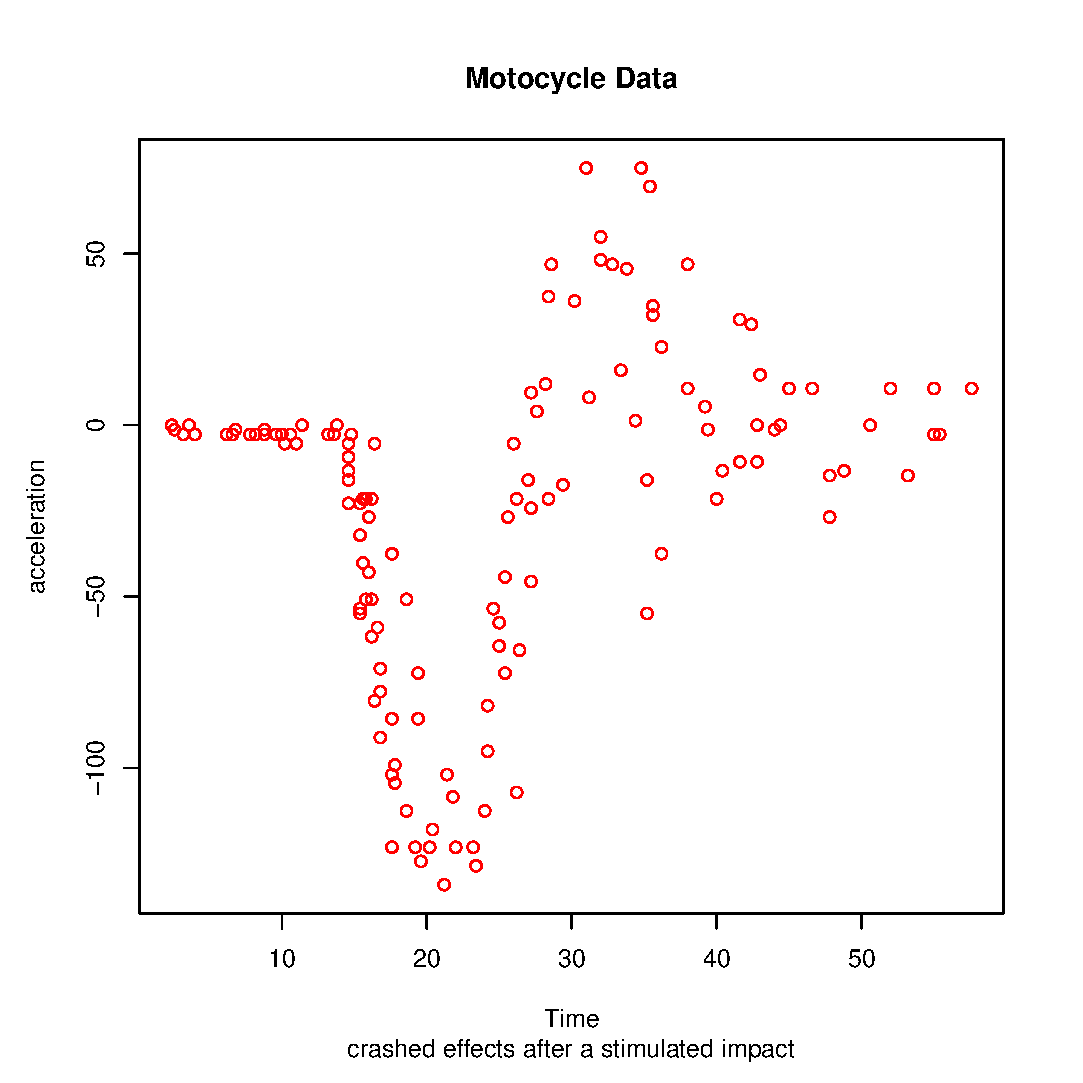
\includegraphics[width=0.75\textwidth,height=0.52\textwidth]{MotocycleData.eps}
    \label{figure2} 

% \end{minipage}
\end{figure}

\newpage
{\LARGE{\textbf{Parametric Modeling}}}
\vskip25pt
{\Large\bf{Polynomial Fit}}

\begin{figure}[h]
% \begin{minipage}[t]{1\linewidth}
\centering
    %the four numbers after "trim=" are for left bottom right top
      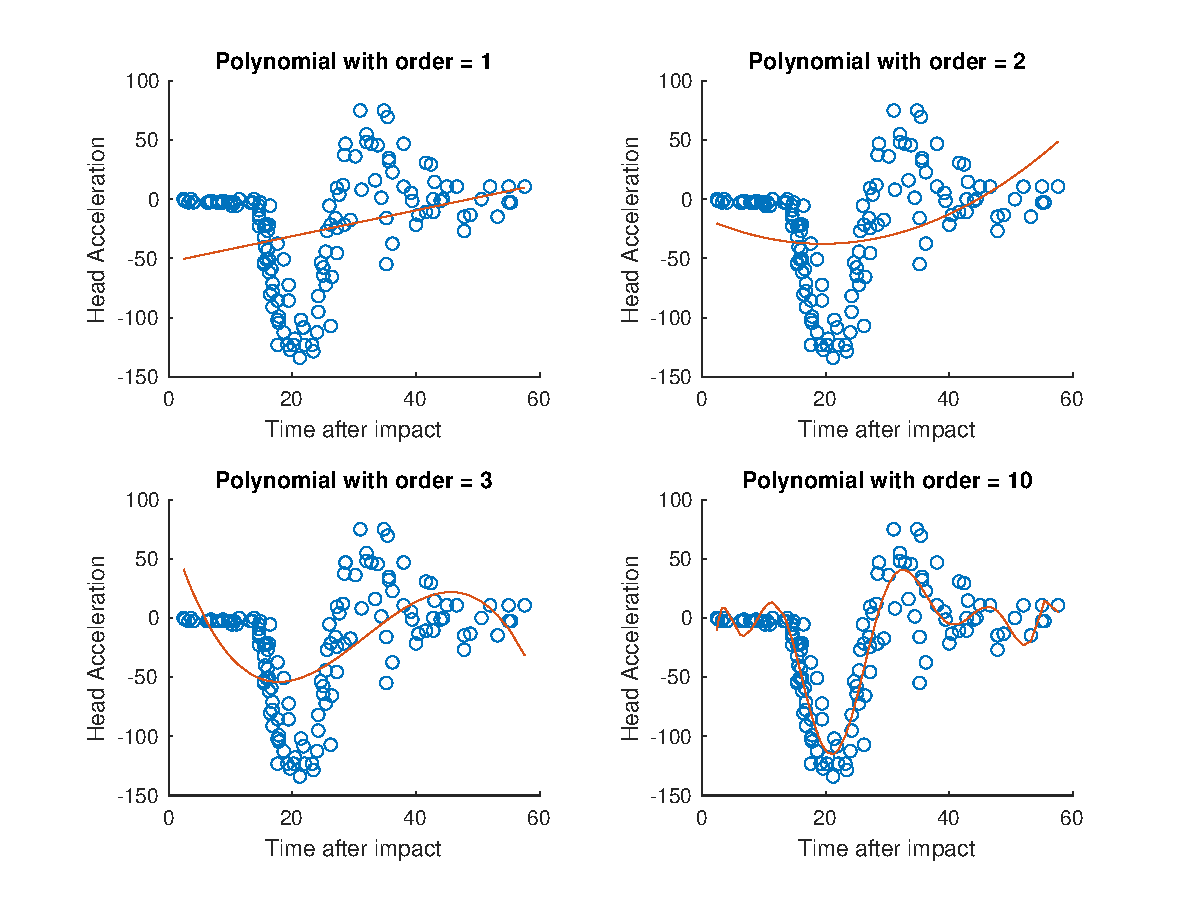
\includegraphics[width=0.75\textwidth,height=0.52\textwidth]{polyfitting.eps}
    \label{figure2} 

% \end{minipage}
\end{figure}

\newpage
{\LARGE\centerline{\textbf{Pros and Cons of nonparametric method}}}
\vskip25pt
\begin{minipage}{.9\textwidth}
    \Large

Nonparametric inference requires weaker assumptions, for instance, 
\vfill
\begin{itemize}
\item $X_1,\dots,X_n$ are i.i.d. and $\E(X_1^2)<\infty$;
\item Or $X_1,\dots,X_n$ are i.i.d. with the $r$-th derivative $f^{(r)}(x)$ of the density exists, for certain $r>0$;
\item No assumptions about specific forms of the density $f$.
\end{itemize}
\end{minipage}

\newpage
{\LARGE\centerline{\textbf{Pros and Cons of nonparametric method}}}
\vskip25pt
\begin{minipage}{.9\textwidth}
    \Large
\begin{itemize}
\item That makes the results more widely applicable and models more robust, i.e. nonparametric regression estimators are very flexible.
\item From the viewpoint of nonparametric approach, all the parametric models are too rigid. 
\item There are situations when a workable parametric model is difficult to establish, for example, in biased sampling. 
\item But their statistical precision decreases greatly if several explanatory variables are included in the model, a.k.a. {\it the curse of dimensionality}.
\end{itemize}

\end{minipage}

\newpage
{\LARGE\centerline{\textbf{Summary}}}
\vskip25pt
\begin{minipage}{.9\textwidth}
    \Large
\begin{itemize}
\item Parametric models are fully determined up to one or more parameters. The statistical accuracy is guaranteed by the correctness of the underlying assumptions. 
\item Nonparametric models avoid using restrictive assumptions of the functional form of the regression function. However, they become difficult to interpret and yield inaccurate estimates if the number of regressors is large. 
\end{itemize}

\end{minipage}

\newpage
{\LARGE\centerline{\textbf{Nonparametric Methods}}}
\vskip25pt
\begin{minipage}{.9\textwidth}
    \Large Can be classified as 
\begin{enumerate}
\item classical nonparametric methods, which are based on signs and ranks developed in 1940s--1970s;
\item modern nonparametric methods, includes:
\begin{itemize}
    \item Smoothing methods, such as kernel, spline, orthogonal series for curve estimation, including density, regression curves. (Note: A curve can be regared as a parameter of infinite dimensions.)
    \item The Jackknife, Bootstrap and other resampling methods. 
\end{itemize}
\end{enumerate}
The course is mostly around the smoothing method and the curves we considered includes the density 
    % $$f(x)=\frac{\mathrm{d}F(x)}{\mathrm{d}x},$$
    and the conditional mean function.
\end{minipage}

\newpage
{\LARGE\centerline{\textbf{A toy example}}}
\vskip25pt
\begin{minipage}{.9\textwidth}
    \Large 
Suppose $\big\{(X_i,Y_i)\big\}_{i=1}^n$ is an i.i.d. sequence, with conditional expectation function
$$m(x)=\E(Y_i|X_i=x)$$ 
and conditional variance $$\sigma^2(x)=\Var(Y_i|X_i=x).$$
Consider the regression 
\begin{equation}\label{L1-eq1}
    Y_i=m(X_i)+\varepsilon_i.
\end{equation}
Apparently, we have 
$$\E(\varepsilon_i|X_i)=0,$$ and
$$\E(\varepsilon_i^2|X_i)=\Var(Y_i|X_i)=\sigma^2(X_i).$$
Besides, $X_i$ and $\varepsilon_i$ are \sout{independent} uncorrelated, i.e. orthogonal in $L^2$.
\end{minipage}

\newpage
{\LARGE\centerline{\textbf{Counterexample}}}
\vskip25pt
\begin{minipage}{.9\textwidth}
    \Large 
    Let $p,p_1,p_2\in(0,1)$ be some constants, and $p_1\ne p_2$. Consider $X,Y$ with following distributions: 
$X\sim Bernoulli(p)$, i.e. 
$$\IP(X=1)=1-\IP(X=0)=p,$$
and $Y\sim Bernoulli(p_1)$ given $X=1$, while $Y\sim Bernoulli(p_2)$ given $X=0$. Therefore, 
$$\E(Y|X)=p_1\cdot X+p_2\cdot(1-X),$$
$$\varepsilon:=Y-\E(Y|X)=Y-[p_1\cdot X+p_2\cdot(1-X)].$$
The conditional distribution of $\varepsilon$ is
$$\IP(\varepsilon=1-p_1|X=1)=1-\IP(\varepsilon=-p_1|X=1)=p_1,$$
and  
$$\IP(\varepsilon=1-p_2|X=0)=1-\IP(\varepsilon=-p_2|X=0)=p_2.$$
\textcolor{red}{$X$ and $\varepsilon$ are not independent, but uncorrelated.}
\end{minipage}

\newpage
{\LARGE\centerline{\textbf{Counterexample(continue)}}}
\vskip25pt
\begin{minipage}{.9\textwidth}
    \Large 
    By the law of total probability, 
    \begin{equation*}
        \varepsilon=\begin{cases}
            1-p_1,~~~&\mathrm{w.p.}~~p_1p,\\
            -p_1,~~~&\mathrm{w.p.}~~(1-p_1)p,\\
            1-p_2,~~~&\mathrm{w.p.}~~p_2(1-p),\\
            -p_2,~~~&\mathrm{w.p.}~~(1-p_2)(1-p),
        \end{cases}
    \end{equation*}
 and  $\E(\varepsilon)=0$. Hence, we have 
   \begin{eqnarray*}
    \cov(X,\varepsilon)&=&\E(X\varepsilon)\\
    &=&p\E(\varepsilon|X=1)\\
    &=&p[(1-p_1)p_1+(-p_1)(1-p_1)]\\
    &=&0.
   \end{eqnarray*}
\end{minipage}









\newpage
\bibliographystyle{apalike}
\bibliography{../ref}
\end{document}